The picking up of sheet metal part is the first step in the automated bending operation. In this phase, the robot arm (KR1410) approaches the raw sheet metal part gripped by the unloading station gripper. The unloading station is equipped with target marker which ensures that the robot reaches the correct scanning position which is perpendicularly over the sheet. (Figure \ref{fig:sheet-pickup})


\begin{figure}[h]
    \centering
    \begin{subfigure}[b]{0.48\textwidth}
        \centering
        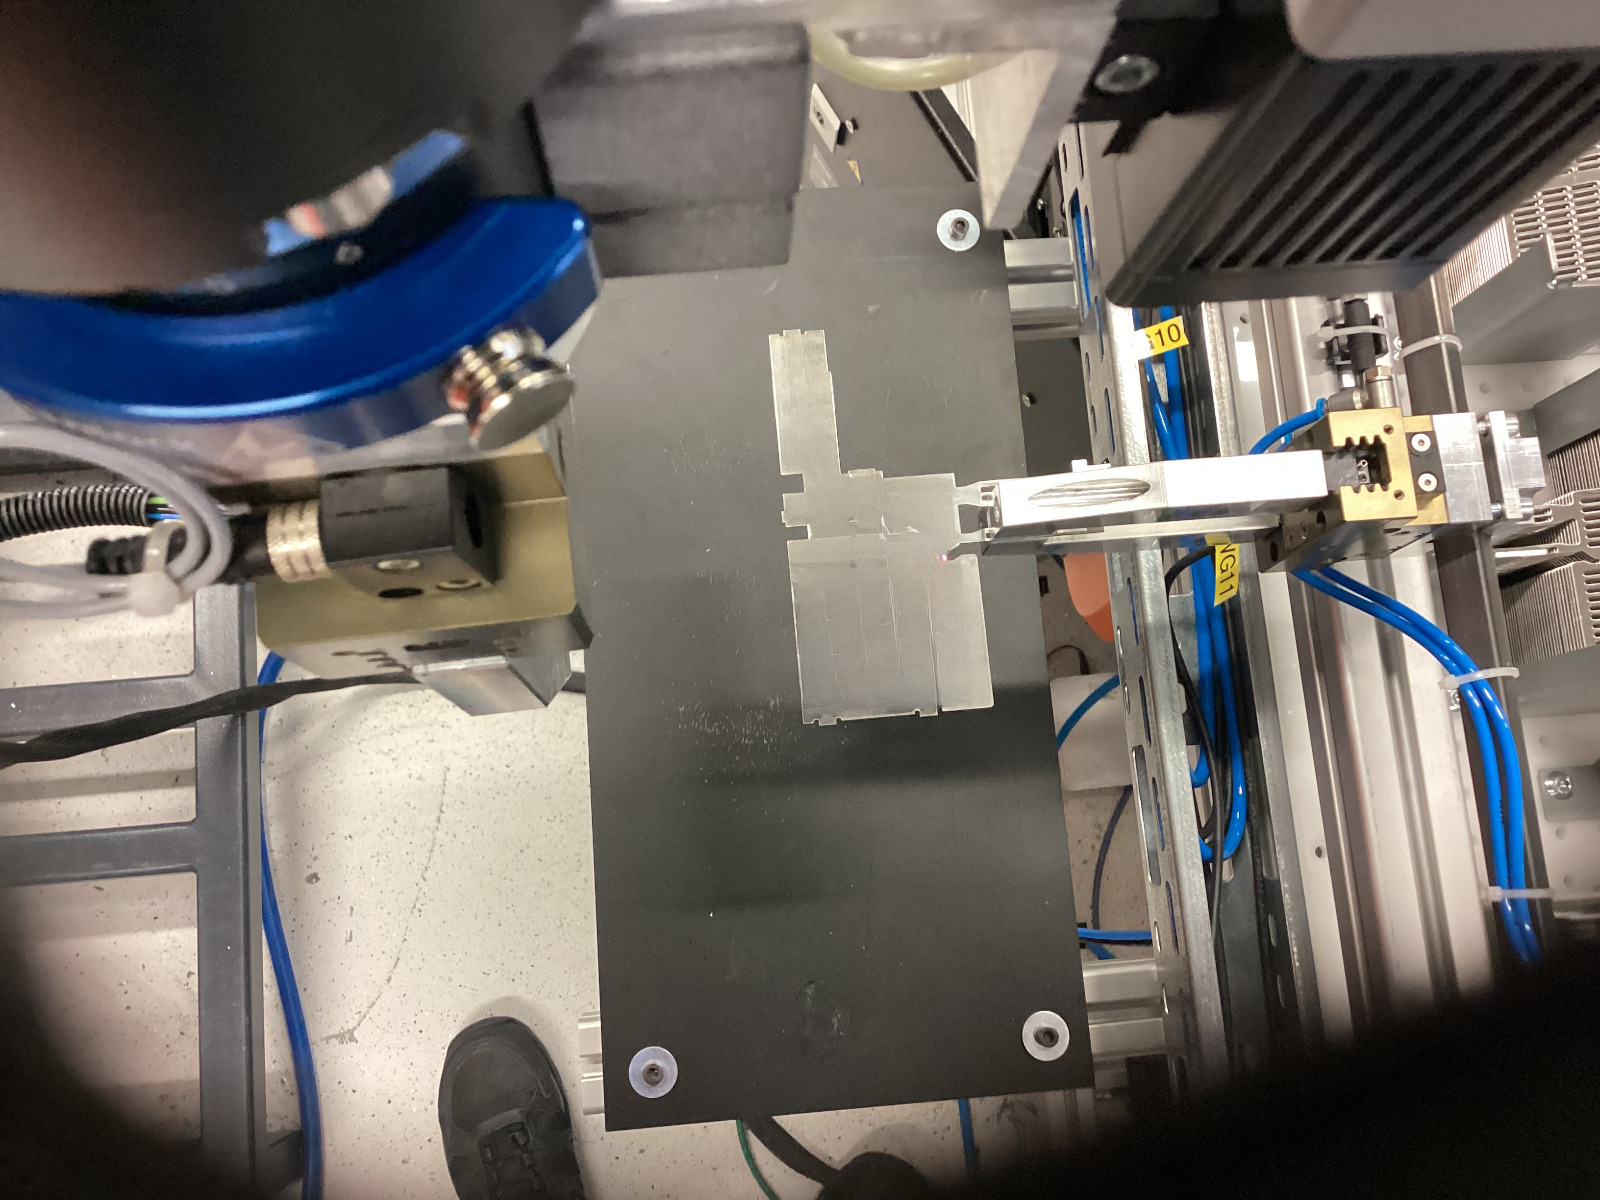
\includegraphics[width=\textwidth]{figures/sheet-pickup/scan.png}
        \caption{Scan sheet pattern using contour detector}
        \label{subfig:sheet-scan}
    \end{subfigure}\hspace{0.1cm}
    \begin{subfigure}[b]{0.48\textwidth}
        \centering
        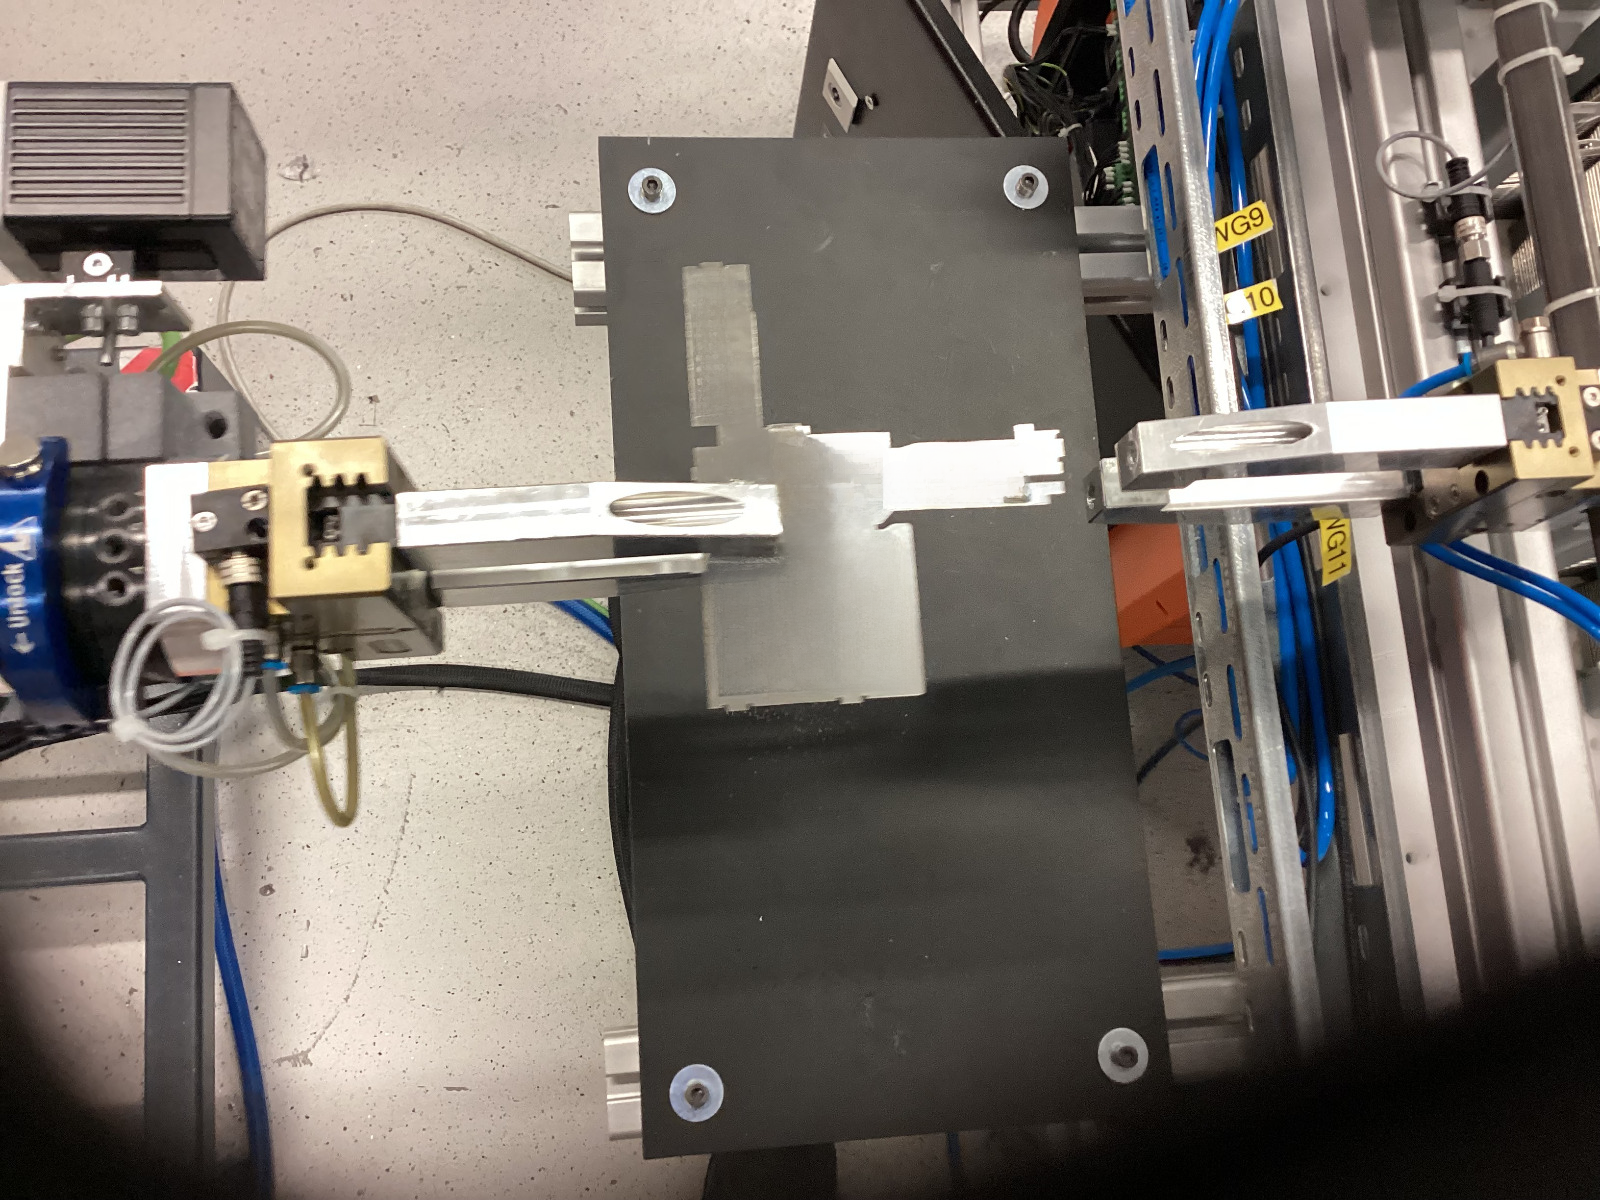
\includegraphics[width=\textwidth]{figures/sheet-pickup/taken.png}
        \caption{collect the sheet}
        \label{subfig:sheet-taken}
    \end{subfigure}
    \caption{Sheet pickup using robotic gripper}
    \label{fig:sheet-pickup}
\end{figure}

\begin{figure}[h]
    \centering
    \begin{subfigure}[b]{0.48\textwidth}
        \centering
        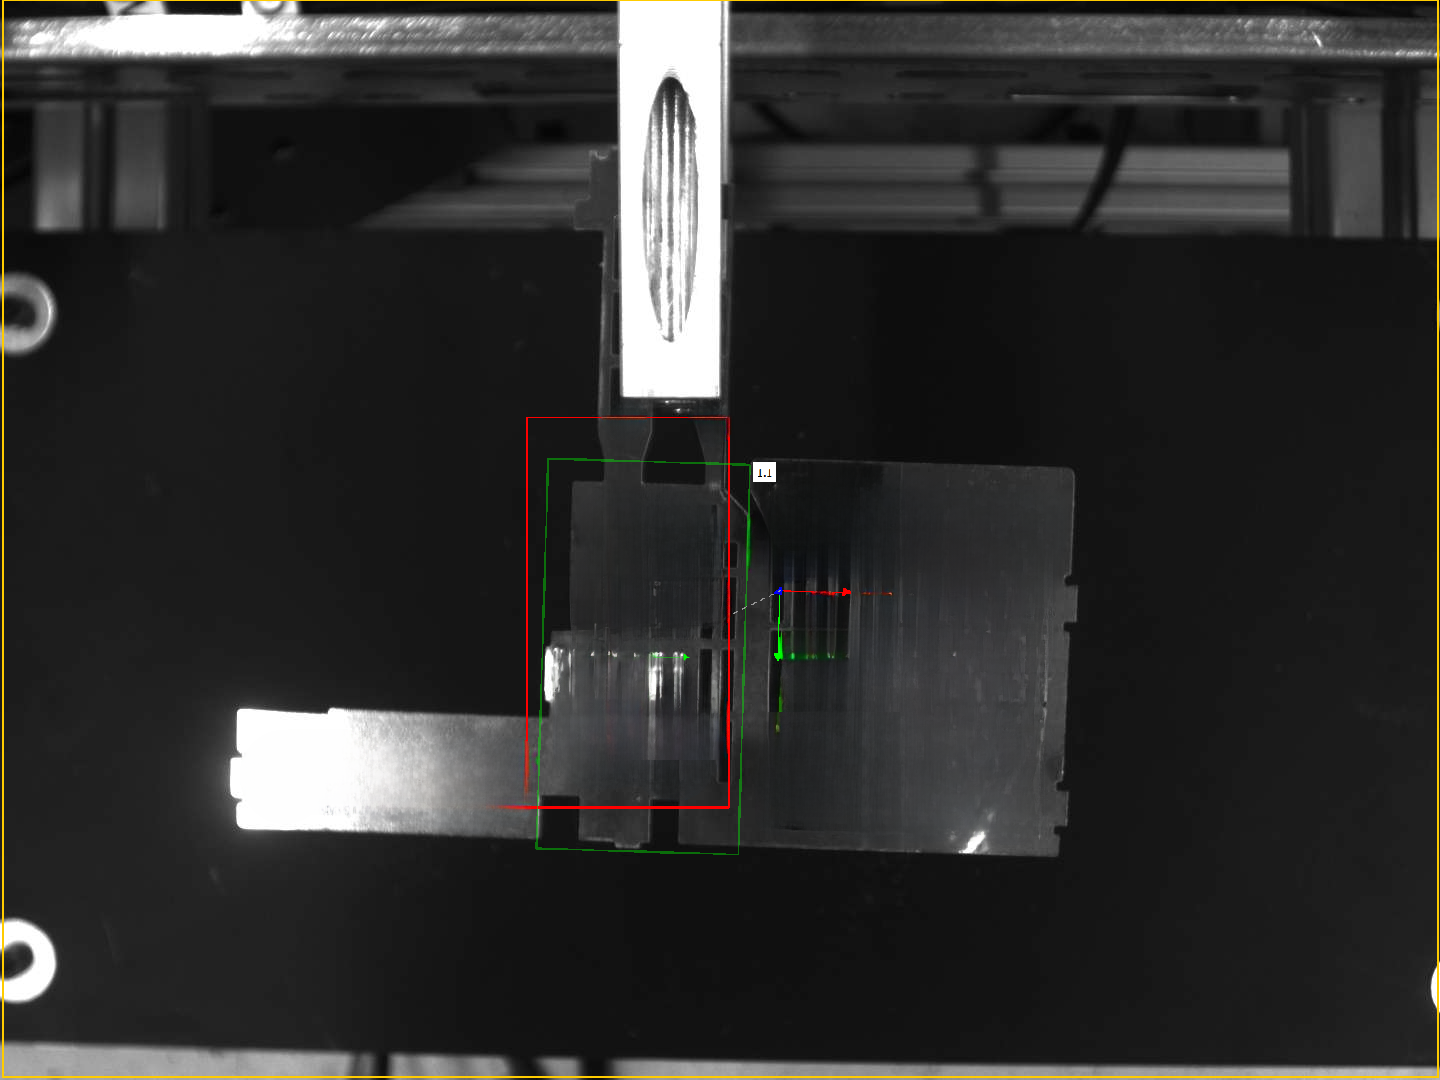
\includegraphics[width=\textwidth]{figures/sheet-pickup/camera-align.png}
        \caption{align camera}
        \label{subfig:sheet-1}
    \end{subfigure}\hspace{0.1cm}
    \begin{subfigure}[b]{0.48\textwidth}
        \centering
        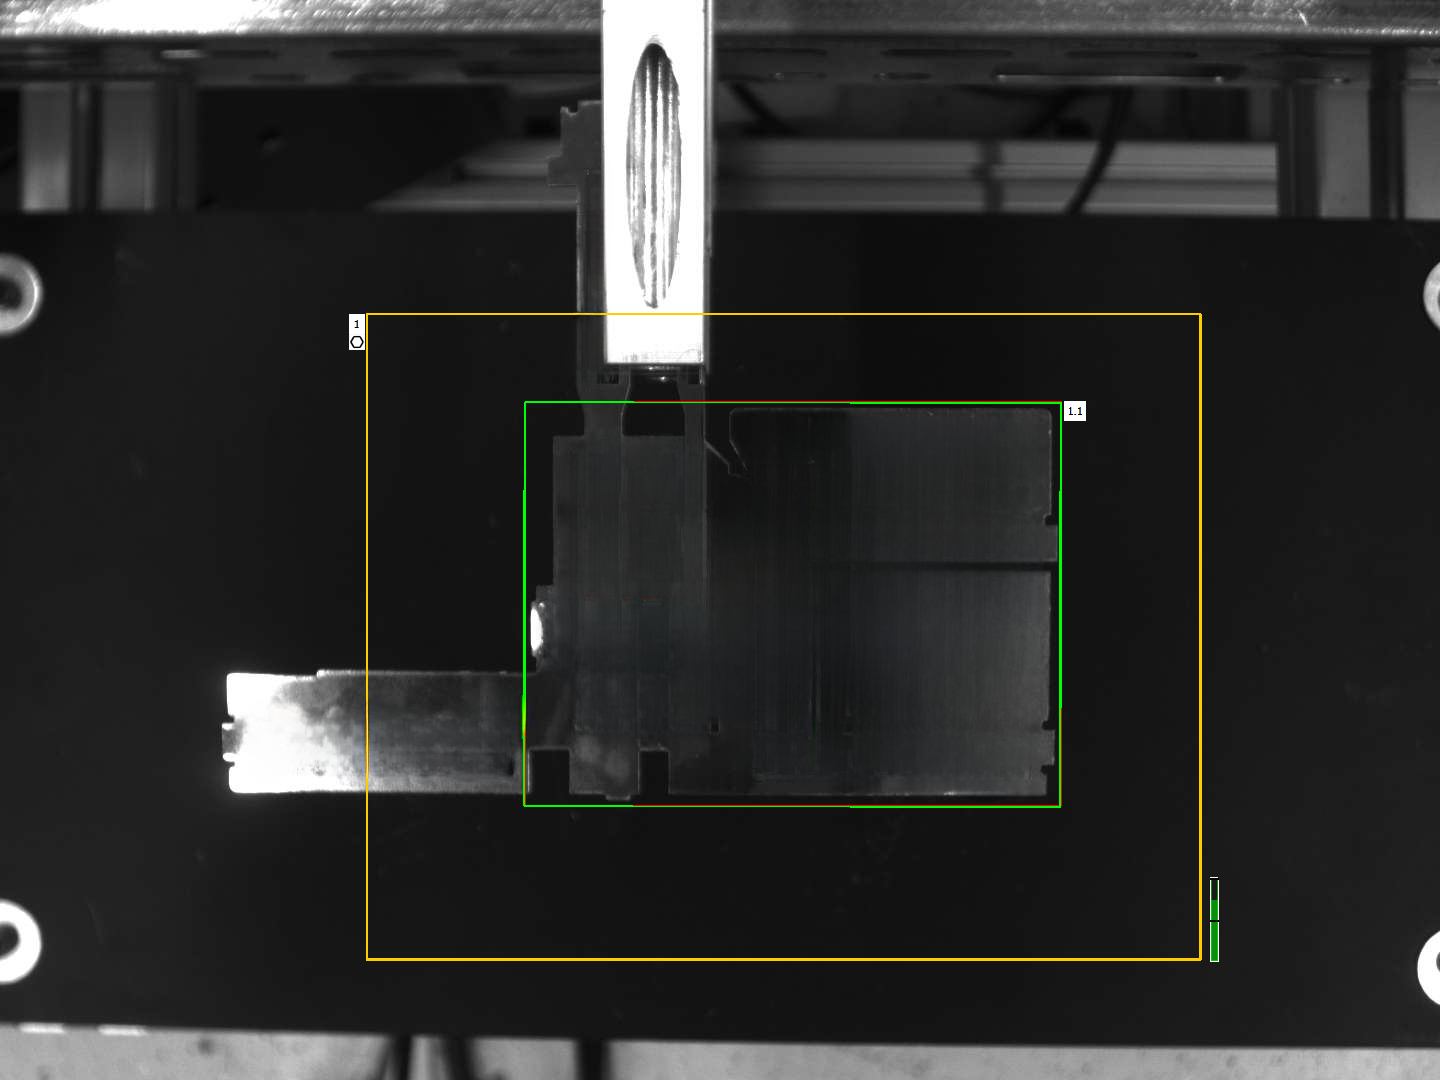
\includegraphics[width=\textwidth]{figures/sheet-pickup/sheet-pose.png}
        \caption{send sheet pose to pickup the sheet}
        \label{subfig:sheet-0}
    \end{subfigure}
    \caption{Sheet pattern detection using detector contour}
    \label{fig:sheet-scanning}
\end{figure}

The KR1410 uses the camera to detect and then securely pick the sheet. There are two stages of scanning as shown in figure \ref{fig:sheet-scanning}. A first scan aligns the camera perfectly with the sheet pattern. The second image capture detects the sheet with high accuracy in this way and sends the pose to the robot in world frame as shown in figure \ref{fig:sensoconfig-pattern}. Both stages uses detector contour to get the sheet pose.
The accuracy of the pickup is crucial for the success of the subsequent bending operations. Any misalignment at this stage could lead to errors in the final dimensions of the bent part.

\begin{figure}[h]
    \centering
    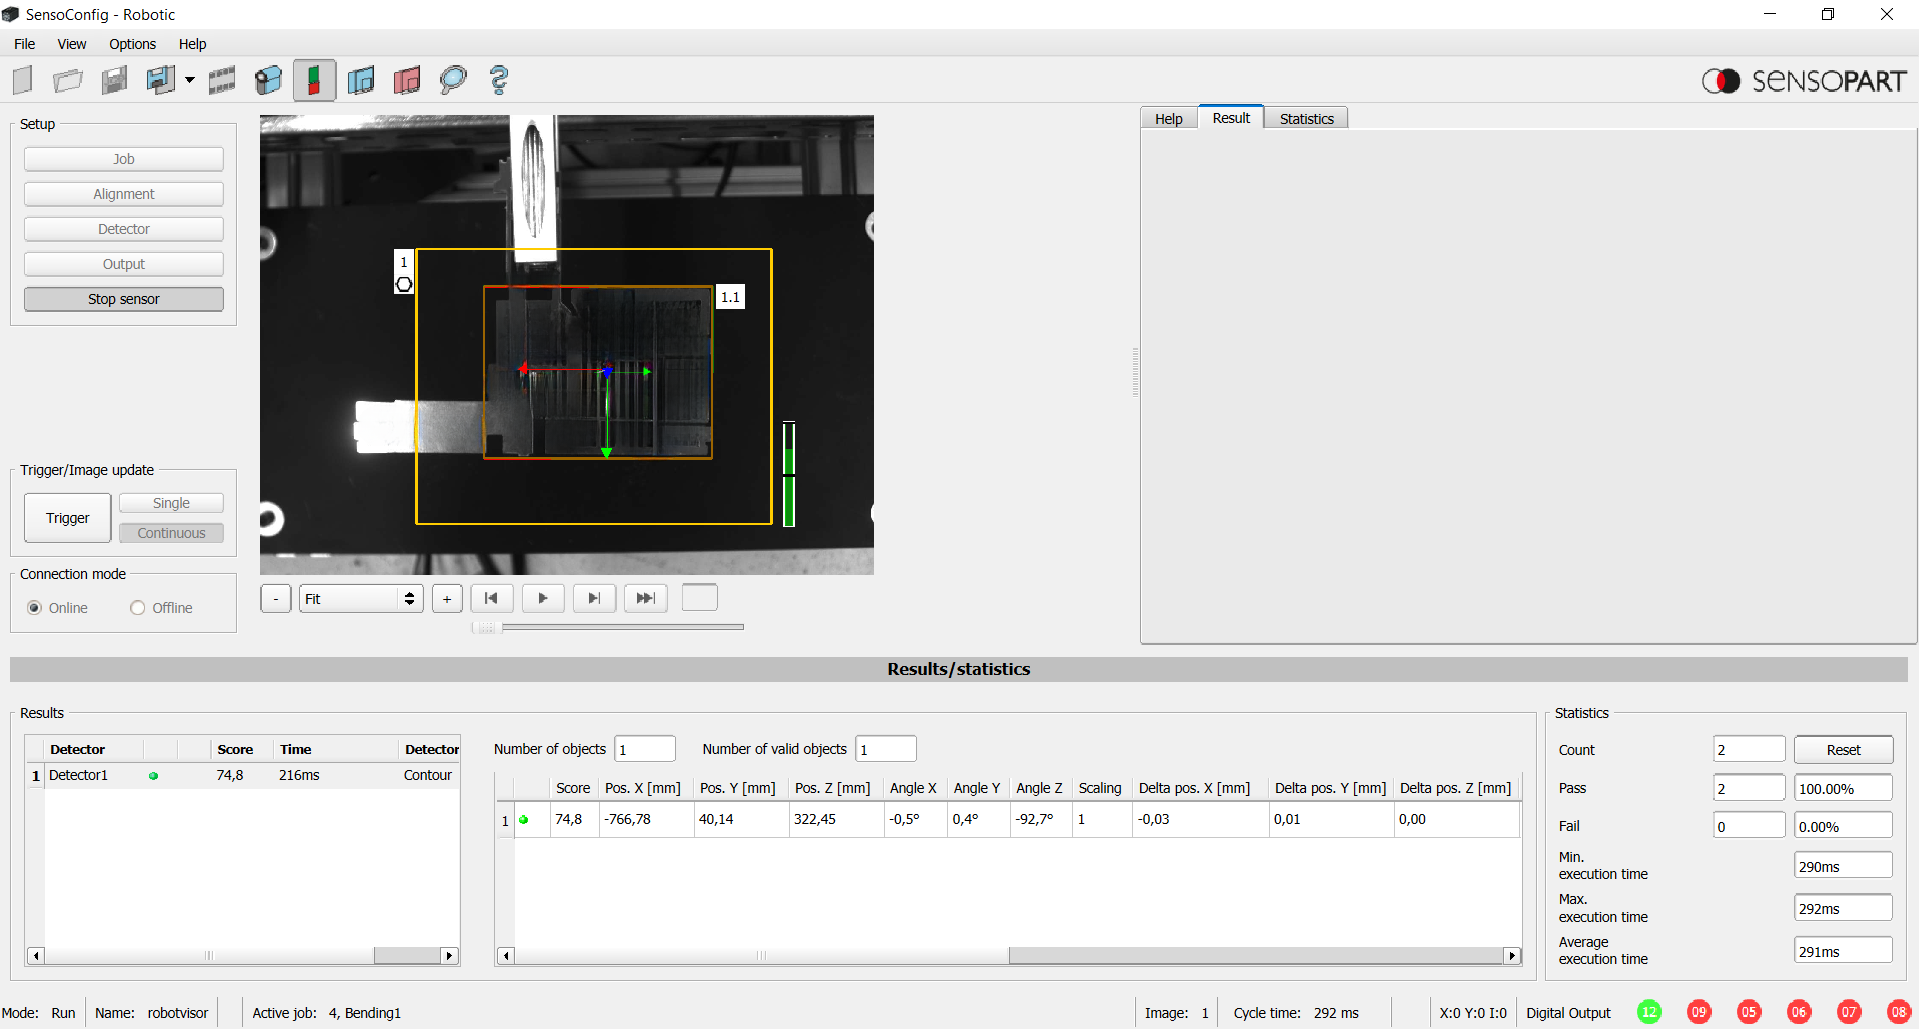
\includegraphics[width=\textwidth]{figures/sheet-pickup/sensoconfig.PNG}
    \caption{Detection and sending of sheet pose using telegram (SensoConfig)}
    \label{fig:sensoconfig-pattern}
\end{figure}

In some instances, to avoid collisions during next bending operation or for better handling of part, regripping of the sheet from a different position is required. This is where the unloading station gripper plays a crucial role in repositioning the sheet. The unloading station gripper is controlled from the KR1410 robot if the robot program state Int[0] is $\ge$3. (See table \ref{tab:kr1410-to-plc}). Otherwise the unloading station gripper is controlled by the PLC. 
\vspace{1\baselineskip}

First, the robot transfers the bent sheet to the unloading station gripper. Then, it is the same process as the sheet pickup in the first step of the bending cycle. The robot moves to the scanning pose, scans and aligns with the sheet, detects and grips the sheet and finally move out the part from the unloading station gripper.
Figure \ref{fig:sheet-pickup-before-placement} illustrates the step-by-step process of regrasping of sheet metal part for sheet placement in the storage station after all the bending operations are complete.


\begin{figure}[h]
    \centering
    \begin{subfigure}[b]{0.32\textwidth}
        \centering
        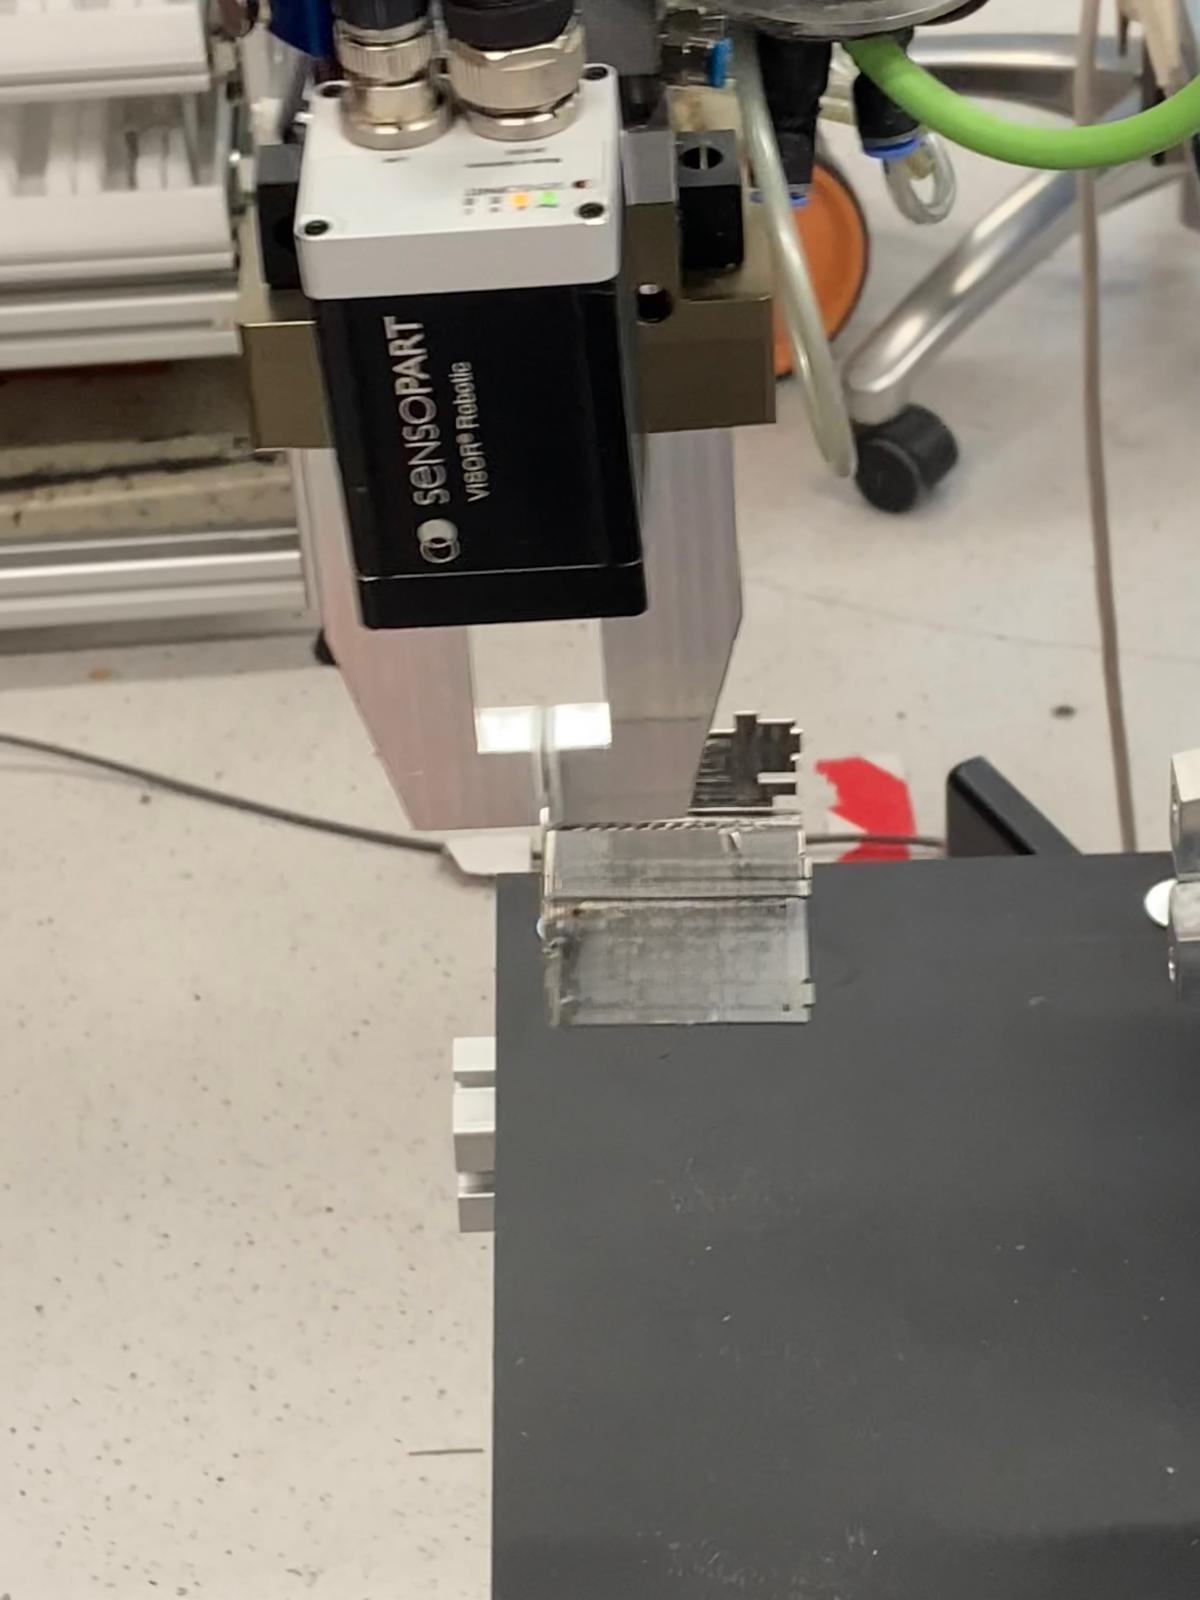
\includegraphics[width=\textwidth]{figures/sheet-pickup/sheet-placement01.png}
        \caption{Go to unloading station gripper}
        \label{subfig:sheet-placement01}
    \end{subfigure}\hspace{0.1cm}
    \begin{subfigure}[b]{0.32\textwidth}
        \centering
        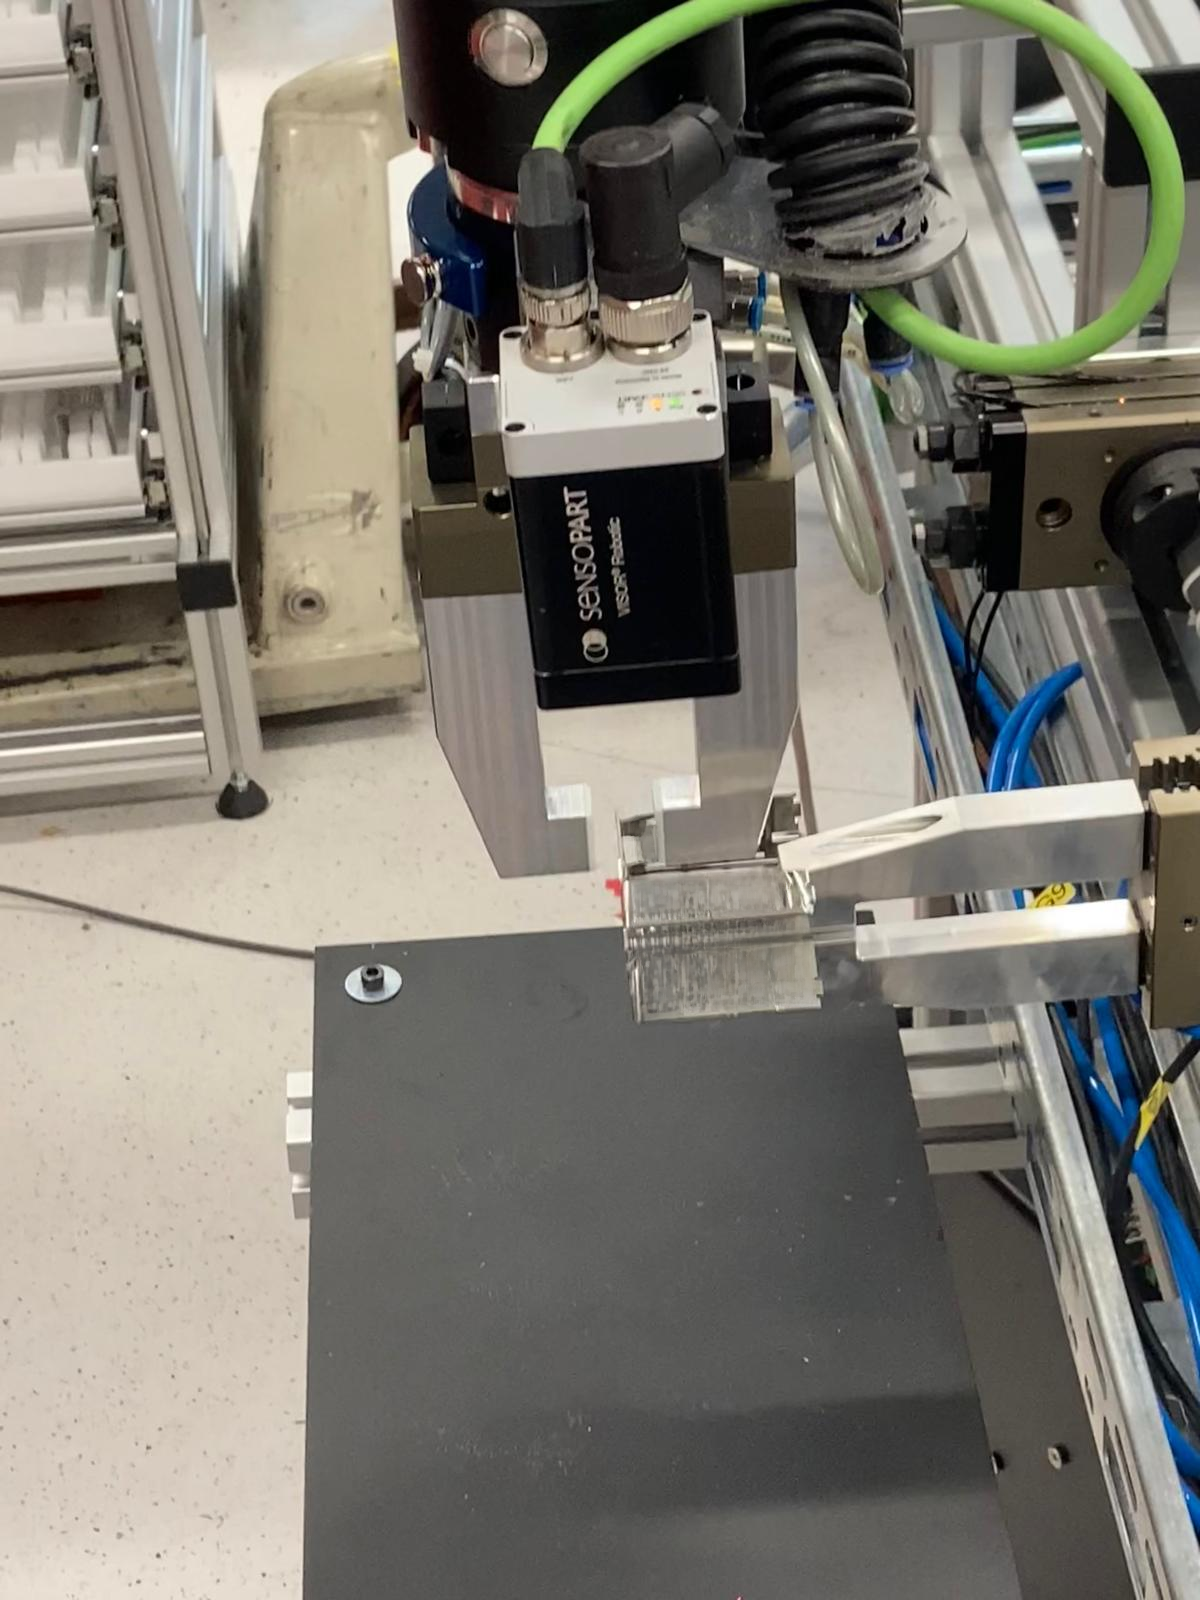
\includegraphics[width=\textwidth]{figures/sheet-pickup/sheet-placement02.png}
        \caption{transfer sheet to unloading station gripper}
        \label{subfig:sheet-placement02}
    \end{subfigure}\hspace{0.1cm}
    \vspace{1cm}
    \begin{subfigure}[b]{0.32\textwidth}
        \centering
        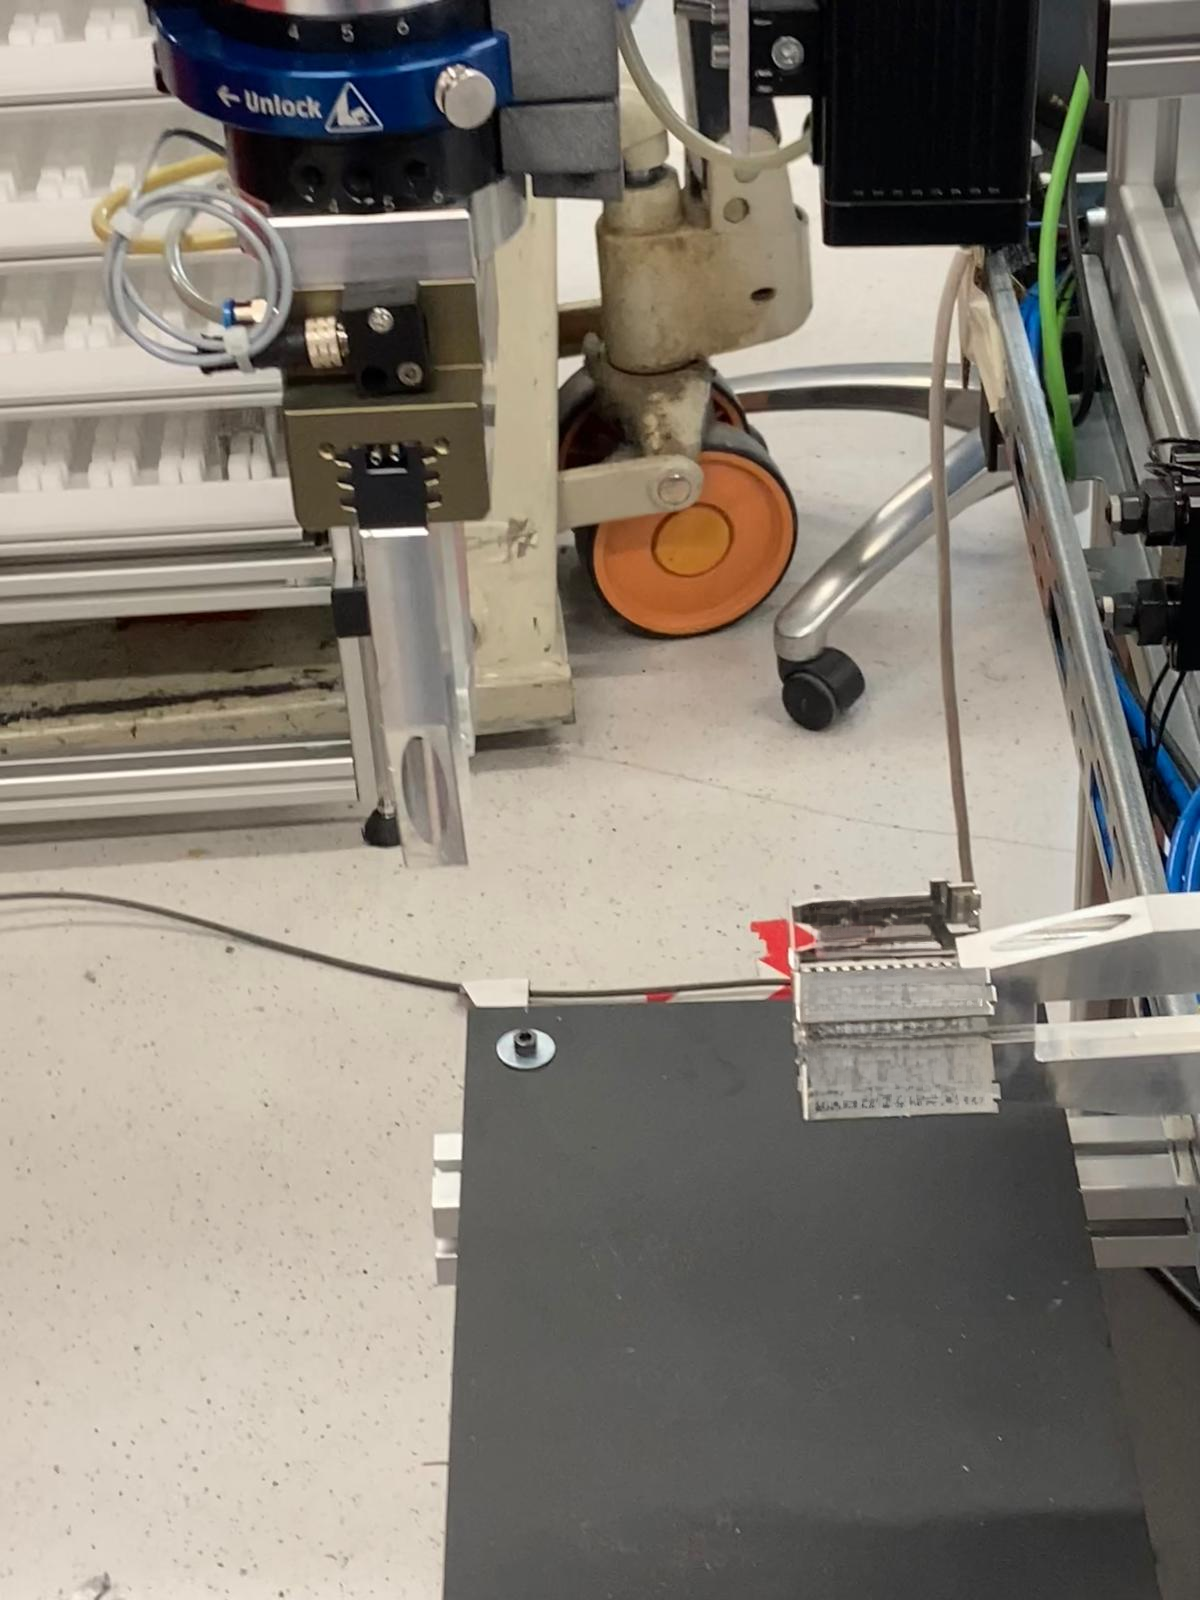
\includegraphics[width=\textwidth]{figures/sheet-pickup/sheet-placement03.png}
        \caption{Scan sheet pattern and align camera}
        % \vspace{-0.45cm}
        \label{subfig:sheet-placement03}
    \end{subfigure}\hspace{0.1cm}
    \begin{subfigure}[b]{0.32\textwidth}
        \centering
        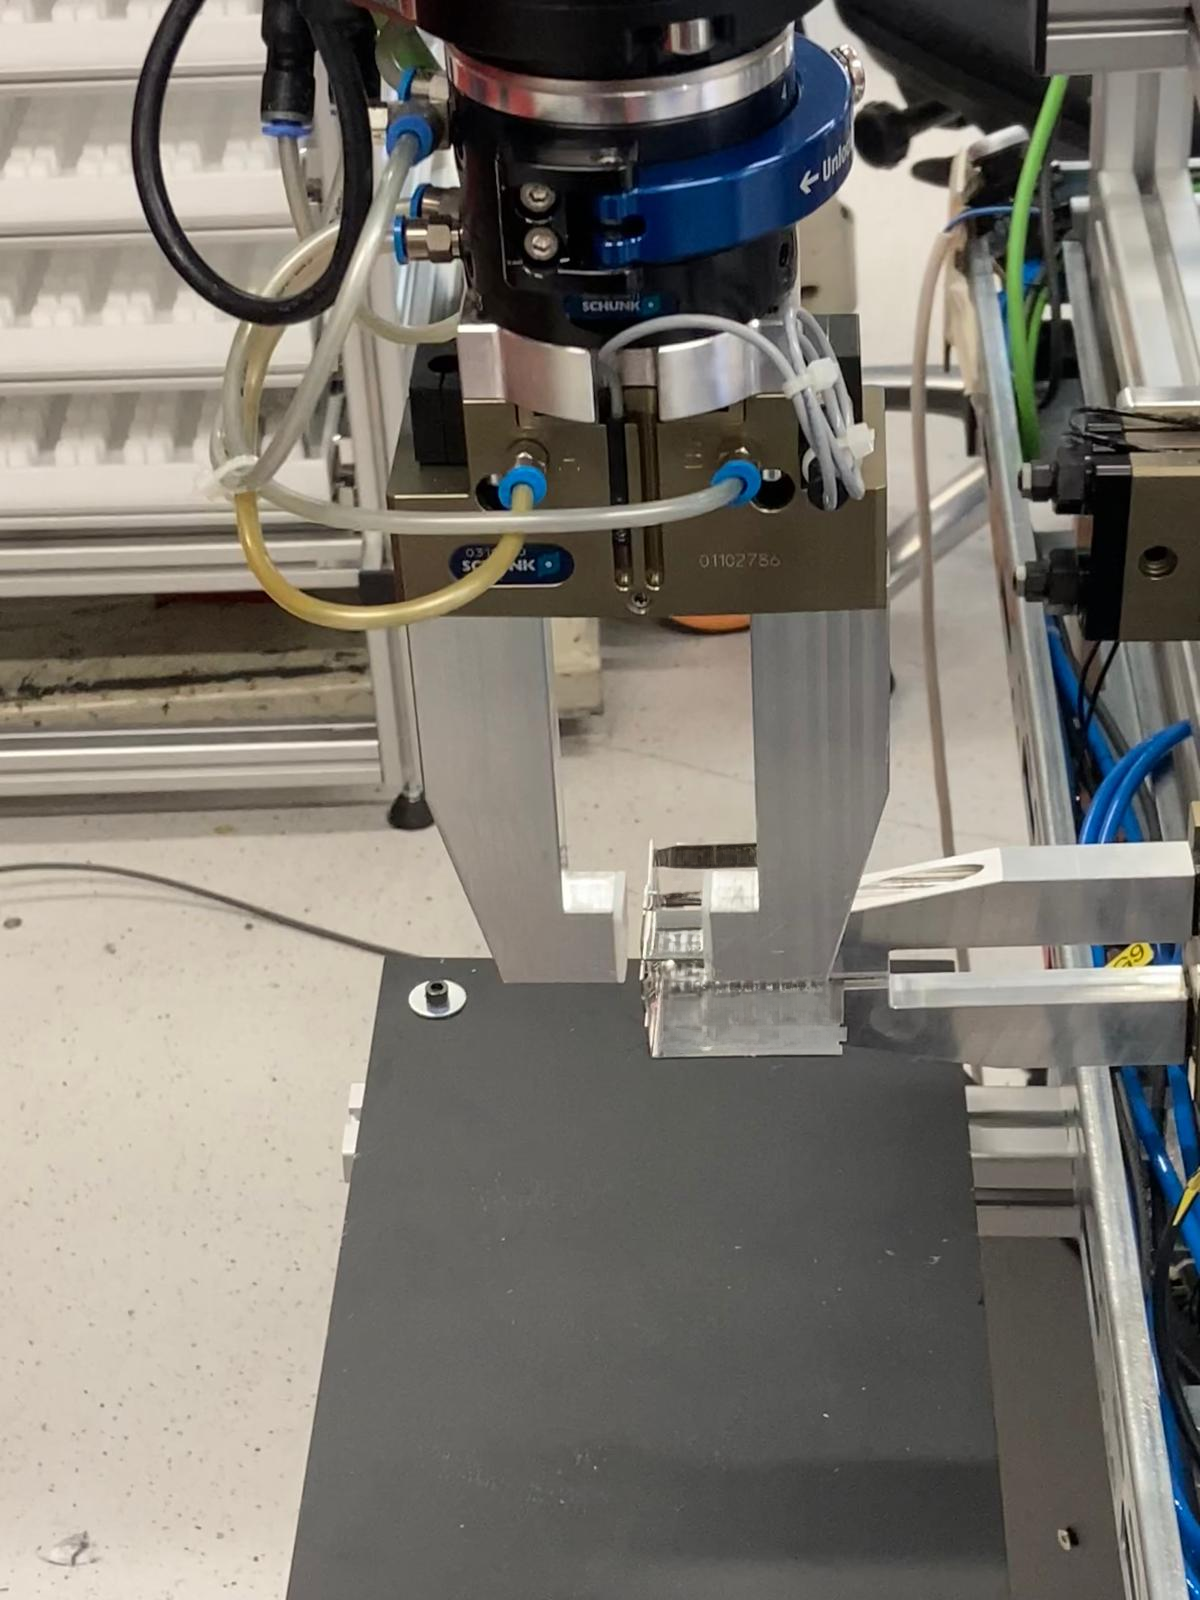
\includegraphics[width=\textwidth]{figures/sheet-pickup/sheet-placement04.png}
        \caption{Scan again for sheet detection}
        \label{subfig:sheet-placement04}
    \end{subfigure}\hspace{0.1cm}
    \vspace{0.75cm}
    \begin{subfigure}[b]{0.32\textwidth}
        \centering
        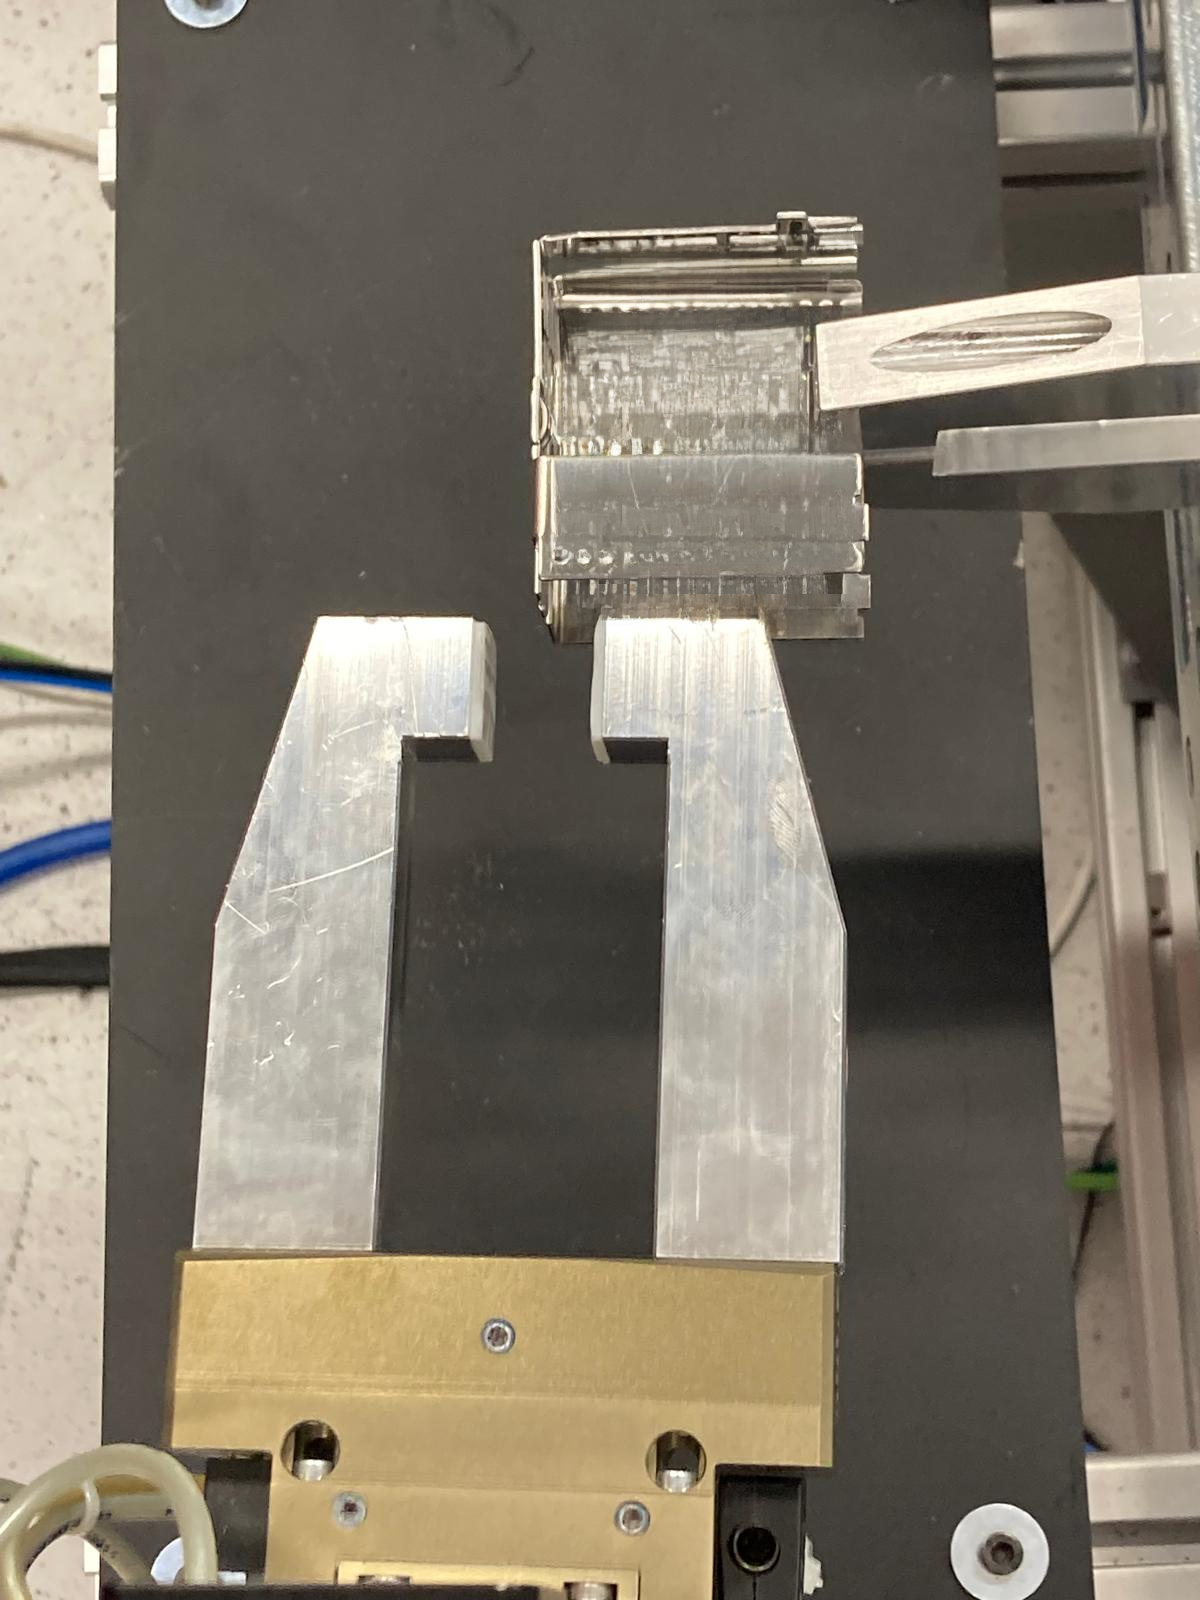
\includegraphics[width=\textwidth]{figures/sheet-pickup/sheet-placement05.png}
        \caption{Grasp sheet from unloading station gripper}
        \label{subfig:sheet-placement05}
    \end{subfigure}\hspace{0.1cm}
    \begin{subfigure}[b]{0.32\textwidth}
        \centering
        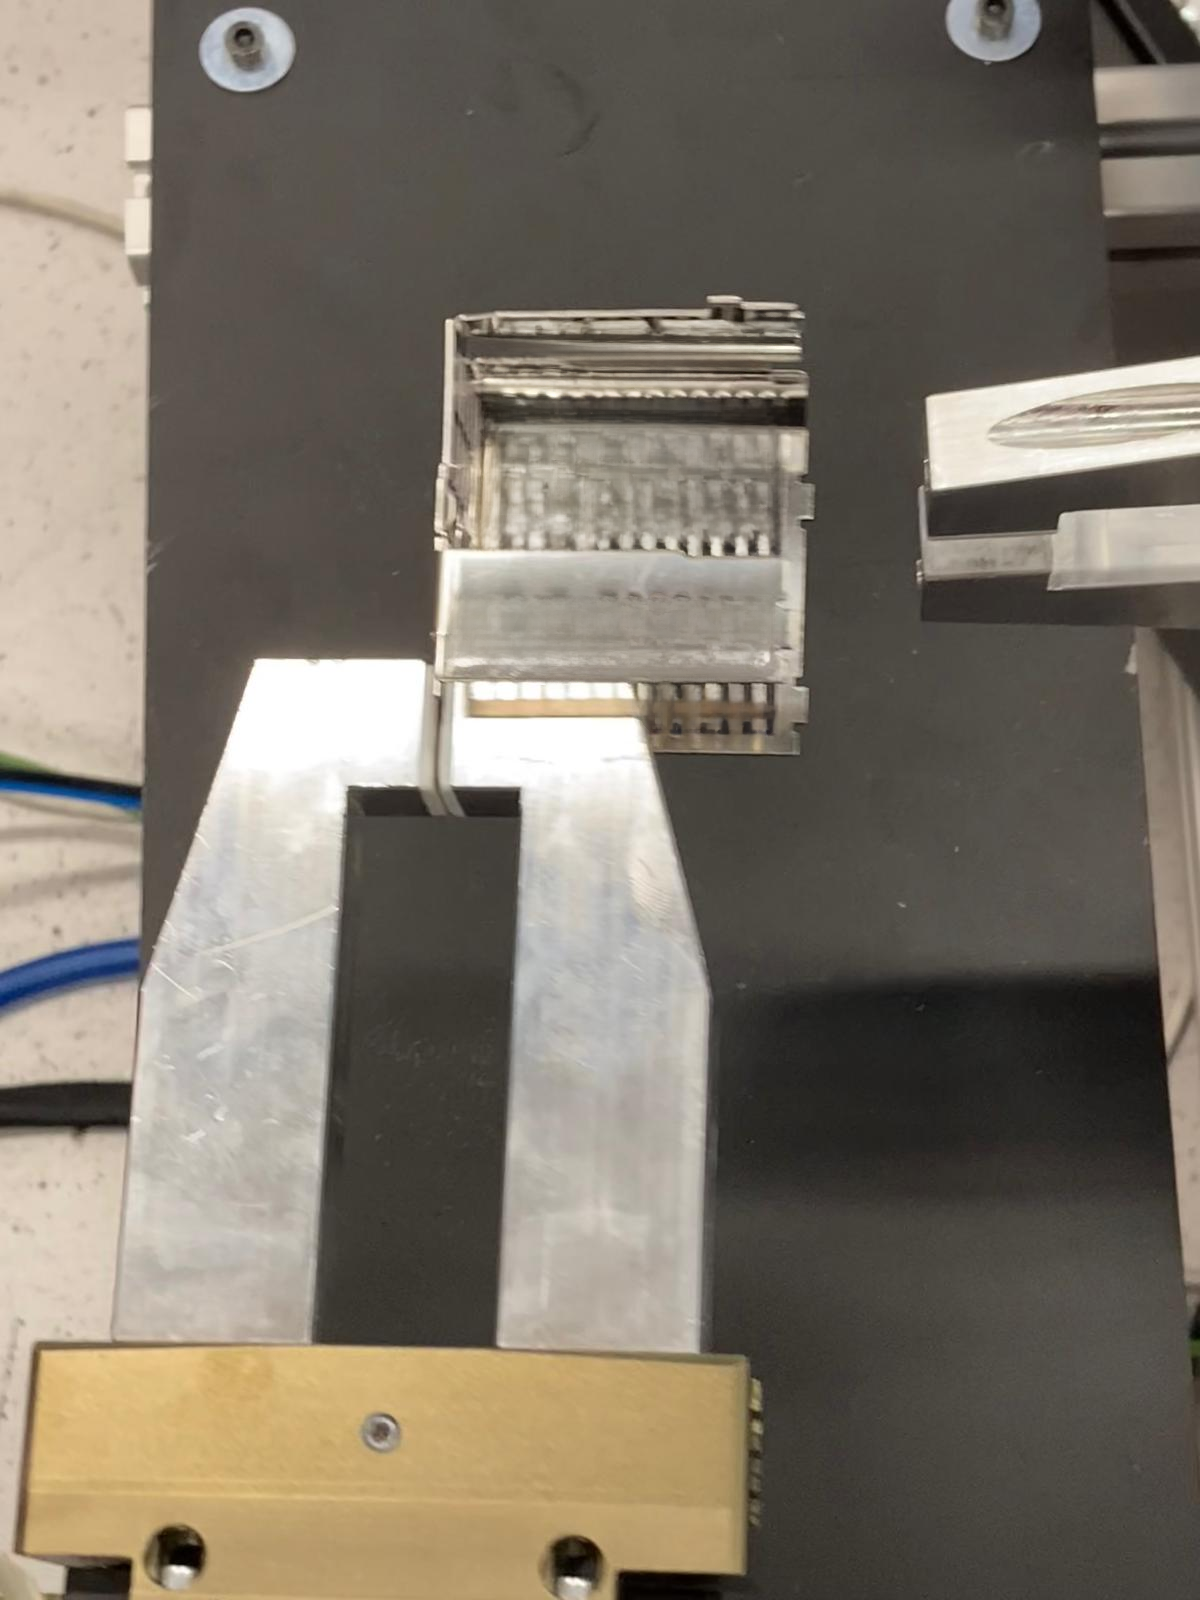
\includegraphics[width=\textwidth]{figures/sheet-pickup/sheet-placement06.png}
        \caption{Move out}
        \label{subfig:sheet-placement06}
        \vspace{0.45cm}
    \end{subfigure}\hspace{0.1cm}
    \caption{Regrasping bent sheet from a different position before placement in drawer}
    \label{fig:sheet-pickup-before-placement}
\end{figure}
